%% Short data paper template
%% Created by Simon Hengchen and Nilo Pedrazzini for the Journal of Open Humanities Data (https://openhumanitiesdata.metajnl.com)

\documentclass{article}
\usepackage[indonesian]{babel}
\usepackage[utf8]{inputenc}
\usepackage{johd}
\usepackage{lipsum}

\title{Analisis Efektivitas Program Penyebaran Bantuan Sosial dalam Upaya Penanggulangan Kemiskinan di Provinsi Bengkulu}

\author{Kevin Synagogue Panjaitan$^{1}$$^{*}$,Alysa Marsellia$^{2}$$^{*}$  \\
        \small $^{a}$ Falkultas Sains Dan Teknologi,Universitas Jambi
        \\\\
        \small $^{*}$Corresponding author: Kevin Synagogue Panjaitan \tt{kpanjaitan123@gmail.com} \\
}
\date{}

\begin{document}
\maketitle


\begin{abstract} 
\noindent 

Kemiskinan masih menjadi tantangan utama di Provinsi Bengkulu. Berbagai program bantuan sosial telah digulirkan pemerintah untuk mengatasinya, namun efektivitasnya belum sepenuhnya jelas. Untuk itu, penelitian ini menganalisis efektivitas penyebaran bantuan sosial dengan menggunakan tiga indikator utama: Rata-Rata Lama Sekolah (RLS), Pengeluaran Per Kapita, dan Upah Minimum Regional (UMR). Ketiga indikator ini dianggap mewakili aspek pendidikan dan ekonomi yang berkaitan erat dengan kemiskinan. Berbagai studi sebelumnya menunjukkan bahwa peningkatan RLS berdampak pada penurunan angka kemiskinan karena pendidikan memperbesar peluang kerja dan pendapatan. Pengeluaran per kapita mencerminkan daya beli masyarakat, yang juga berhubungan dengan kesejahteraan. Sementara itu, UMR dapat meningkatkan pendapatan pekerja dan berkontribusi dalam pengurangan kemiskinan, meskipun dampaknya bisa bervariasi antar wilayah. Penelitian ini menggunakan metode \textit{K-Means Clustering} untuk mengelompokkan kabupaten/kota di Provinsi Bengkulu berdasarkan ketiga indikator tersebut. Data diambil dari Badan Pusat Statistik (BPS) dan mencakup 10 wilayah. Hasil analisis menunjukkan bahwa titik optimal jumlah klaster adalah tiga. Visualisasi dan klasterisasi mengungkap bahwa daerah dengan RLS dan pengeluaran lebih tinggi cenderung berada dalam klaster yang berbeda dibandingkan dengan daerah yang lebih rendah pada kedua indikator tersebut. Sebagai contoh, Kota Bengkulu tergolong dalam klaster dengan tingkat pendidikan dan ekonomi tertinggi. Sementara itu, kabupaten seperti Kaur dan Seluma berada dalam klaster dengan indikator yang lebih rendah. Perbedaan ini menunjukkan bahwa kondisi sosial ekonomi di Provinsi Bengkulu sangat bervariasi, sehingga kebijakan bantuan sosial sebaiknya disesuaikan dengan karakteristik tiap klaster. Dengan pendekatan berbasis data ini, program pengentasan kemiskinan dapat lebih tepat sasaran dan efisien.



 \end{abstract}


\noindent\keywords{Kemiskinan, Bantuan Sosial, Rata-Rata Lama Sekolah, Pengeluaran Per Kapita, Upah Minimum Regional, K-Means Clustering, Provinsi Bengkulu}
\\

% \noindent\authorroles{For determining author roles, please use following taxonomy: \url{https://credit.niso.org/}. Please list the roles for each author.}\\

% \noindent{Data papers have a word limit of 1,000-1,500 words, excluding title, author affiliations, abstract, Tables/Figures and references, but including Tables/Figures captions and footnotes. To complete this data paper template, please delete or replace the text not given in bold with your own text.} \\

% \noindent{Authors must ensure that the manuscript text, including the abstract, is original and not directly taken from dataset repository descriptions. The text must be paraphrased and adapted to fit the context of the article.}

\section{Pendahuluan}

Kemiskinan merupakan salah satu tantangan utama yang dihadapi oleh banyak negara, termasuk Indonesia. Provinsi Bengkulu, dengan karakteristik geografis dan demografis yang unik, menghadapi permasalahan kemiskinan yang kompleks. Dalam upaya menurunkan angka kemiskinan, pemerintah telah meluncurkan berbagai program bantuan sosial yang bertujuan meningkatkan kesejahteraan masyarakat. Namun, efektivitas program-program tersebut sering kali dipertanyakan, terutama ketika dikaitkan dengan indikator pendidikan dan ekonomi sebagai tolok ukur keberhasilan penanggulangan kemiskinan. Salah satu cara untuk menilai efektivitas tersebut adalah dengan menganalisis beberapa indikator, seperti Rata-Rata Lama Sekolah (RLS), Pengeluaran Per Kapita, dan Upah Minimum Regional (UMR).



Rata-Rata Lama Sekolah (RLS) merupakan salah satu indikator penting yang memengaruhi tingkat kemiskinan. Semakin tinggi rata-rata lama sekolah, semakin besar peluang masyarakat untuk keluar dari lingkaran kemiskinan. Beberapa penelitian mendukung temuan ini. \cite{pradipta2020pengaruh} menemukan bahwa RLS memiliki pengaruh negatif yang signifikan terhadap kemiskinan, artinya setiap kenaikan RLS berdampak pada penurunan tingkat kemiskinan. Hasil serupa juga ditunjukkan oleh \cite{permatasari2024analisis} yang menganalisis pengaruh pendidikan, termasuk RLS, terhadap kemiskinan di Jawa. Penelitian di daerah lain pun memberikan hasil konsisten, seperti ditunjukkan oleh \cite{samudra2023pengaruh} di Provinsi D, serta \cite{supriyadi2024ketimpangn} yang menekankan bahwa peningkatan pendidikan mampu menekan kemiskinan sekaligus mengurangi dampak sosial negatif, termasuk ketimpangan.


Selain faktor pendidikan, pengeluaran per kapita juga merupakan salah satu indikator penting yang berpengaruh terhadap tingkat kemiskinan. Beberapa penelitian menunjukkan bahwa peningkatan pengeluaran per kapita dapat membantu menekan angka kemiskinan. 

Misalnya, \cite{muttaqin2025elastisitas} menemukan bahwa elastisitas kemiskinan terhadap pertumbuhan pengeluaran per kapita di Jawa Barat menunjukkan hubungan negatif, artinya peningkatan pengeluaran per kapita berbanding lurus dengan penurunan angka kemiskinan. Penelitian lain yang dilakukan oleh \cite{siregar2023analisis} juga memperkuat temuan tersebut dengan menyatakan bahwa pengeluaran per kapita berpengaruh negatif dan signifikan terhadap kemiskinan. 

\cite{rabbani2025analisis} menambahkan bahwa pengeluaran per kapita, bersama dengan pendidikan dan kesehatan, memberikan pengaruh positif dan signifikan terhadap penurunan tingkat kemiskinan. Selain itu, \cite{nugroho2020leading} menekankan bahwa pengeluaran per kapita merupakan salah satu data utama dalam perhitungan angka kemiskinan, sehingga indikator ini memiliki peranan yang sangat penting dalam menentukan status kemiskinan suatu wilayah.


Lebih lanjut, Upah Minimum Regional (UMR) juga terbukti berpengaruh signifikan terhadap tingkat kemiskinan. Sejumlah penelitian internasional menegaskan hal tersebut. Misalnya,\cite{munguia2024minimum} menunjukkan bahwa peningkatan upah minimum di Meksiko pada periode 2019–2022 mampu menurunkan jumlah penduduk miskin sebesar 23,7\% hingga 37,6\%. Penelitian lain oleh \cite{dantas2025non} menyatakan bahwa upah minimum lebih efektif dalam mengurangi insiden kemiskinan dibandingkan kedalaman kemiskinan, sehingga kenaikan upah minimum berimplikasi signifikan terhadap penurunan angka kemiskinan. \cite{alaniz2011impact} juga menemukan bahwa peningkatan upah minimum berkontribusi terhadap pengurangan kemiskinan dan ketimpangan pendapatan melalui peningkatan upah bagi kelompok pekerja yang terdampak. Meskipun demikian, \cite{bassier2024can}. mencatat bahwa dampak upah minimum terhadap kemiskinan di negara berkembang cenderung relatif kecil. Namun, peningkatan upah minimum tetap dapat memberikan manfaat nyata, khususnya bagi kelompok pekerja berpenghasilan rendah.


Artikel ini bertujuan untuk menganalisis efektivitas program penyebaran bantuan sosial di Provinsi Bengkulu dengan menggunakan data Rata-Rata Lama Sekolah, Pengeluaran Per Kapita, dan Upah Minimum Regional (UMR) di kabupaten-kabupaten di provinsi tersebut. Rata-Rata Lama Sekolah menjadi indikator penting dalam menilai kualitas pendidikan dan potensi sumber daya manusia, sementara Pengeluaran Per Kapita mencerminkan tingkat kesejahteraan ekonomi masyarakat. UMR, di sisi lain, memberikan gambaran tentang standar upah yang diterima oleh pekerja di daerah tersebut.

Melalui analisis ini, diharapkan dapat diperoleh pemahaman yang lebih mendalam mengenai dampak program bantuan sosial terhadap pengurangan kemiskinan di Provinsi Bengkulu. Dengan demikian, hasil penelitian ini diharapkan dapat memberikan rekomendasi yang konstruktif bagi pengambil kebijakan dalam merancang program-program yang lebih efektif dan berkelanjutan.



% \section{Metodologi Penelitian}

% \subsection{Desain Penelitian}
% Penelitian ini menggunakan pendekatan kuantitatif dengan desain deskriptif dan analitis. Tujuan utama dari penelitian ini adalah untuk menganalisis efektivitas program penyebaran bantuan sosial dalam penanggulangan kemiskinan di Provinsi Bengkulu, sebagaimana diuraikan dalam Bab 1. Dengan memanfaatkan data statistik yang relevan, penelitian ini bertujuan untuk memberikan pemahaman yang lebih mendalam mengenai dampak program bantuan sosial terhadap indikator-indikator sosial dan ekonomi.

% \subsection{Lokasi dan Waktu Penelitian}
% Penelitian ini dilakukan di Provinsi Bengkulu, dengan fokus pada kabupaten-kabupaten yang terdapat di provinsi tersebut. Pengumpulan data dilakukan selama periode [masukkan periode waktu, misalnya: Januari 2025 hingga Maret 2025], yang mencakup waktu di mana program bantuan sosial dilaksanakan.

% \subsection{Data dan Sumber Data}
% Data yang digunakan dalam penelitian ini meliputi:
% \begin{itemize}
%     \item \textbf{Rata-Rata Lama Sekolah (RLS)}: Data ini mencerminkan tingkat pendidikan masyarakat di setiap kabupaten, yang berhubungan langsung dengan pengurangan kemiskinan, seperti yang dijelaskan dalam Bab 1.
%     \item \textbf{Pengeluaran Per Kapita}: Data ini menunjukkan rata-rata pengeluaran per individu di setiap kabupaten, yang merupakan indikator kesejahteraan ekonomi dan berkontribusi pada penurunan tingkat kemiskinan.
%     \item \textbf{Upah Minimum Regional (UMR)}: Data ini memberikan gambaran tentang standar upah yang diterima oleh pekerja di daerah tersebut, yang berpengaruh signifikan terhadap tingkat kemiskinan.
% \end{itemize}

% Sumber data diperoleh dari [sebutkan sumber data, misalnya: Badan Pusat Statistik (BPS), Dinas Sosial Provinsi Bengkulu, dan lembaga terkait lainnya].

% \subsection{Metode Analisis Data}
% Metode analisis yang digunakan dalam penelitian ini adalah analisis kluster dengan teknik K-Means. Langkah-langkah analisis adalah sebagai berikut:

% \begin{enumerate}
%     \item \textbf{Persiapan Data}: Data yang diperoleh akan dibersihkan dan dipersiapkan untuk analisis. Ini termasuk penanganan data yang hilang dan normalisasi data agar berada dalam skala yang sama.
    
%     \item \textbf{Pemilihan Variabel}: Variabel yang digunakan dalam analisis K-Means adalah Rata-Rata Lama Sekolah, Pengeluaran Per Kapita, dan UMR. Variabel-variabel ini dipilih karena relevansinya dalam menggambarkan kondisi kemiskinan dan efektivitas program bantuan sosial, seperti yang telah dibahas dalam Bab 1.
    
%     \item \textbf{Penentuan Jumlah Kluster}: Sebelum melakukan analisis K-Means, jumlah kluster yang optimal akan ditentukan menggunakan metode Elbow atau Silhouette.
    
%     \item \textbf{Pelaksanaan K-Means}: Setelah jumlah kluster ditentukan, algoritma K-Means akan diterapkan untuk mengelompokkan kabupaten-kabupaten berdasarkan variabel yang telah dipilih. Proses ini akan menghasilkan beberapa kluster yang menunjukkan tingkat efektivitas program bantuan sosial.

%     Persamaan matematis untuk K-Means adalah sebagai berikut:

%     \begin{equation}
%     J = \sum_{i=1}^{k} \sum_{j=1}^{n} \| x_j^{(i)} - \mu_i \|^2
%     \end{equation}

%     Di mana:
%     \begin{itemize}
%         \item \( J \) adalah fungsi objektif yang ingin diminimalkan (jumlah kuadrat jarak antara titik data dan pusat kluster).
%         \item \( k \) adalah jumlah kluster.
%         \item \( n \) adalah jumlah titik data.
%         \item \( x_j^{(i)} \) adalah titik data ke-j dalam kluster ke-i.
%         \item \( \mu_i \) adalah pusat kluster ke-i.
%     \end{itemize}

%     \item \textbf{Interpretasi Hasil}: Hasil klustering akan dianalisis untuk mengidentifikasi karakteristik masing-masing kluster dan hubungannya dengan efektivitas program bantuan sosial dalam penanggulangan kemiskinan. Dengan mengelompokkan kabupaten-kabupaten berdasarkan RLS, Pengeluaran Per Kapita, dan UMR, penelitian ini bertujuan untuk mengidentifikasi wilayah yang paling membutuhkan bantuan sosial.
% \end{enumerate}

% \subsection{Validitas dan Reliabilitas}
% Untuk memastikan validitas dan reliabilitas data, penelitian ini akan menggunakan triangulasi data dengan membandingkan hasil analisis K-Means dengan data kualitatif yang diperoleh dari wawancara dengan pihak terkait, seperti pengelola program bantuan sosial dan masyarakat penerima bantuan. Hal ini penting untuk memastikan bahwa hasil penelitian dapat diandalkan dan mencerminkan kondisi nyata di lapangan.







\section{Landasan Teori}

Kemiskinan merupakan fenomena kompleks yang dipengaruhi oleh berbagai faktor, termasuk pendidikan, ekonomi, dan kebijakan sosial. Dalam konteks Provinsi Bengkulu, beberapa indikator penting yang digunakan untuk menganalisis kemiskinan adalah Rata-Rata Lama Sekolah (RLS), Pengeluaran Per Kapita, dan Upah Minimum Regional (UMR).

\subsection{Rata-Rata Lama Sekolah (RLS)}

Rata-Rata Lama Sekolah (RLS) adalah indikator yang mencerminkan tingkat pendidikan masyarakat. Pendidikan yang lebih tinggi berhubungan dengan peningkatan kemampuan individu untuk mendapatkan pekerjaan yang lebih baik dan meningkatkan pendapatan. Penelitian oleh \cite{pradipta2020pengaruh} menunjukkan bahwa RLS memiliki pengaruh negatif yang signifikan terhadap kemiskinan, di mana setiap kenaikan RLS berkontribusi pada penurunan tingkat kemiskinan.

\subsection{Pengeluaran Per Kapita}

Pengeluaran Per Kapita adalah ukuran yang menunjukkan rata-rata pengeluaran individu dalam suatu wilayah. Peningkatan pengeluaran per kapita dapat berkontribusi pada penurunan angka kemiskinan. Penelitian oleh \cite{muttaqin2025elastisitas} menemukan bahwa terdapat hubungan negatif antara pertumbuhan pengeluaran per kapita dan kemiskinan, yang menunjukkan bahwa peningkatan pengeluaran per kapita berbanding lurus dengan penurunan angka kemiskinan.

\subsection{Upah Minimum Regional (UMR)}

Upah Minimum Regional (UMR) adalah standar upah terendah yang ditetapkan oleh pemerintah. Kenaikan UMR diharapkan dapat meningkatkan pendapatan pekerja dan mengurangi kemiskinan. Penelitian oleh \cite{munguia2024minimum} menunjukkan bahwa peningkatan upah minimum di Meksiko mampu menurunkan jumlah penduduk miskin secara signifikan. Hal ini menunjukkan bahwa UMR memiliki peranan penting dalam penanggulangan kemiskinan.



\subsection{K-Means Clustering}
K-Means adalah algoritma yang digunakan untuk mengelompokkan objek berdasarkan atribut menjadi beberapa cluster, di mana setiap cluster berisi objek yang memiliki karakteristik serupa . Proses ini termasuk dalam kategori unsupervised classification, di mana tidak ada label yang diberikan untuk data, sehingga fokusnya adalah pada pemahaman pola dalam cluster .

Langkah-langkah dalam algoritma K-Means meliputi:

\begin{enumerate}
   \item Menentukan jumlah cluster yang diinginkan.

   \item Menentukan nilai centroid awal secara acak .

   \item Menghitung jarak antara centroid dan setiap objek menggunakan rumus Euclidean Distance .

    \item Mengelompokkan objek berdasarkan jarak minimum ke centroid.

    \item Mengulangi proses hingga tidak ada perubahan dalam anggota cluster.

\end{enumerate}
   
Kelemahan dari K-Means termasuk ketidakmampuan untuk menentukan jumlah cluster yang optimal tanpa pengetahuan sebelumnya dan ketidakpastian dalam kontribusi atribut dalam pengelompokan. Meskipun demikian, K-Means tetap menjadi metode yang sederhana dan efektif untuk menyelesaikan masalah pengelompokan data.



\subsection{Data dan Sumber Data}

Data yang digunakan dalam penelitian ini mencakup Rata-Rata Lama Sekolah, Pengeluaran Per Kapita, dan Upah Minimum Regional di kabupaten-kabupaten di Provinsi Bengkulu. Sumber data diperoleh dari Badan Pusat Statistik (BPS) Provinsi Bengkulu, yang dapat diakses melalui \url{https://bengkulu.bps.go.id/id} Data yang dikumpulkan akan mencakup periode terbaru yang tersedia untuk memberikan gambaran yang akurat mengenai kondisi kemiskinan di Provinsi Bengkulu.

\subsection{Metode Analisis}

Metode analisis yang digunakan dalam penelitian ini adalah klustering dengan algoritma K-Means. Metode ini dipilih untuk mengelompokkan kabupaten-kabupaten di Provinsi Bengkulu berdasarkan indikator-indikator kemiskinan yang telah disebutkan. Langkah-langkah analisis meliputi:

\begin{enumerate}
    \item Pengumpulan data dari sumber yang telah disebutkan.
    \item Pembersihan dan pengolahan data untuk memastikan kualitas dan konsistensi.
    \item Menentukan jumlah kluster yang optimal menggunakan metode Elbow atau Silhouette.
    \item Melakukan klustering dengan algoritma K-Means untuk mengelompokkan kabupaten berdasarkan RLS, Pengeluaran Per Kapita, dan UMR.
    \item Menganalisis hasil klustering untuk mengidentifikasi pola dan karakteristik masing-masing kelompok kabupaten.
\end{enumerate}

Dengan menggunakan metode analisis ini, diharapkan dapat diperoleh pemahaman yang lebih mendalam mengenai dampak program bantuan sosial terhadap pengurangan kemiskinan di Provinsi Bengkulu serta mengidentifikasi kelompok kabupaten yang memiliki karakteristik serupa dalam konteks kemiskinan.





\subsection{Metode Penelitian}

\subsubsection{Pengolahan Data}
Pengolahan data dilakukan untuk mempersiapkan data yang akan digunakan dalam analisis efektivitas program penyebaran bantuan sosial. Data yang digunakan dalam penelitian ini mencakup Rata-Rata Lama Sekolah, Pengeluaran Per Kapita, dan Upah Minimum Regional (UMR) di kabupaten-kabupaten di Provinsi Bengkulu. Data tersebut diolah menggunakan bahasa pemrograman Python dengan library Pandas.

\subsubsection{Struktur Data}
Data yang digunakan dalam penelitian ini disusun dalam bentuk tabel dengan struktur sebagai berikut:

\begin{table}[h]
    \centering
    \caption{Rata-Rata Lama Sekolah, Pengeluaran Per Kapita, dan UMR per Kabupaten (2020-2024)}
  \begin{tabular}{lccc}
        \hline
        \textbf{Kabupaten} & \textbf{Rata\_Rata\_Lama\_Sekolah} & \textbf{Pengeluaran\_Per\_Kapita} & \textbf{UMR} \\
        \hline
        Bengkulu Selatan & 9.350 & 10353.6 & 2318411.4 \\
        Rejang Lebong & 8.554 & 10667.4 & 2318411.4 \\
        Bengkulu Utara & 8.098 & 10870.0 & 2334301.4 \\
        Kaur & 8.404 & 9069.4 & 2318411.4 \\
        Seluma & 8.070 & 8711.2 & 2318411.4 \\
        Mukomuko & 8.406 & 10831.6 & 2594047.4 \\
        Lebong & 8.216 & 11691.8 & 2318411.4 \\
        Kepahiang & 8.312 & 9804.4 & 2318411.4 \\
        Bengkulu Tengah & 7.532 & 9869.2 & 2410581.4 \\
        Kota Bengkulu & 11.816 & 14603.0 & 2510097.6 \\
        \hline
    \end{tabular}
   
    \label{tab:tabel_kabupaten}
\end{table}


\subsubsection{Proses Pengolahan Data}
Proses pengolahan data dilakukan dengan langkah-langkah sebagai berikut:

\begin{enumerate}
    \item \textbf{Pengumpulan Data}: Data dikumpulkan dari sumber-sumber resmi seperti Badan Pusat Statistik (BPS) dan Dinas Sosial Provinsi Bengkulu.
    
    \item \textbf{Pembersihan Data}: Data yang diperoleh akan dibersihkan dari nilai yang hilang atau tidak valid untuk memastikan kualitas data yang digunakan dalam analisis.
    
    \item \textbf{Normalisasi Data}: Data dinormalisasi agar berada dalam skala yang sama, sehingga memudahkan analisis kluster.
    
    \texttt{hasil\_olah\_data.csv} tanpa menyertakan indeks.
\end{enumerate}
% \section{Interpretasi Data}

% \subsection{Rata-Rata Lama Sekolah}
% \begin{itemize}
%     \item \textbf{Kota Bengkulu} memiliki rata-rata lama sekolah tertinggi (11.816 tahun), menunjukkan bahwa penduduk di kabupaten ini memiliki akses yang lebih baik terhadap pendidikan.
%     \item \textbf{Bengkulu Tengah} memiliki rata-rata lama sekolah terendah (7.532 tahun), yang menunjukkan bahwa pendidikan di kabupaten ini mungkin memerlukan perhatian lebih.
% \end{itemize}

% \subsection{Pengeluaran Per Kapita}
% \begin{itemize}
%     \item \textbf{Kota Bengkulu} juga memiliki pengeluaran per kapita tertinggi (14,603.0), yang menunjukkan bahwa penduduk di kabupaten ini memiliki daya beli yang lebih baik.
%     \item \textbf{Seluma} memiliki pengeluaran per kapita terendah (8,711.2), yang menunjukkan bahwa penduduk di kabupaten ini mungkin menghadapi tantangan ekonomi yang lebih besar.
% \end{itemize}

% \subsection{UMR (Upah Minimum Regional)}
% \begin{itemize}
%     \item UMR di semua kabupaten bervariasi, tetapi terlihat bahwa kabupaten dengan pengeluaran per kapita yang lebih tinggi (seperti Kota Bengkulu) juga memiliki UMR yang lebih tinggi.
%     \item UMR yang lebih tinggi di kabupaten seperti Mukomuko (2,594,047.4) menunjukkan bahwa meskipun pengeluaran per kapita tidak setinggi Kota Bengkulu, ada potensi untuk meningkatkan kesejahteraan penduduk.
% \end{itemize}

% \subsection{Kluster}
% \begin{itemize}
%     \item \textbf{Kluster 0}: Terdiri dari kabupaten Kaur, Seluma, dan Kepahiang, yang memiliki rata-rata lama sekolah dan pengeluaran per kapita yang lebih rendah.
%     \item \textbf{Kluster 1}: Hanya mencakup Kota Bengkulu, yang menunjukkan bahwa kabupaten ini memiliki karakteristik yang sangat berbeda dibandingkan dengan yang lain.
%     \item \textbf{Kluster 2}: Termasuk beberapa kabupaten (Bengkulu Selatan, Rejang Lebong, Bengkulu Utara, dan Lebong) dengan rata-rata lama sekolah dan pengeluaran per kapita yang sedang.
%     \item \textbf{Kluster 3}: Hanya mencakup Mukomuko, yang menunjukkan bahwa kabupaten ini memiliki karakteristik yang unik.
%     \item \textbf{Kluster 4}: Hanya mencakup Bengkulu Tengah, yang menunjukkan bahwa kabupaten ini juga memiliki karakteristik yang berbeda.
% \end{itemize}

% \section{Kesimpulan}
% Data ini menunjukkan adanya variasi yang signifikan dalam tingkat pendidikan, kesejahteraan ekonomi, dan upah minimum di antara kabupaten-kabupaten di provinsi Bengkulu. Klustering membantu mengidentifikasi kelompok kabupaten dengan karakteristik serupa, yang dapat digunakan untuk merancang kebijakan dan program intervensi yang lebih efektif untuk meningkatkan pendidikan dan kesejahteraan di daerah yang membutuhkan.




\section{Hasil Dan Pembahasaan}

\begin{figure}[H]
    \centering
    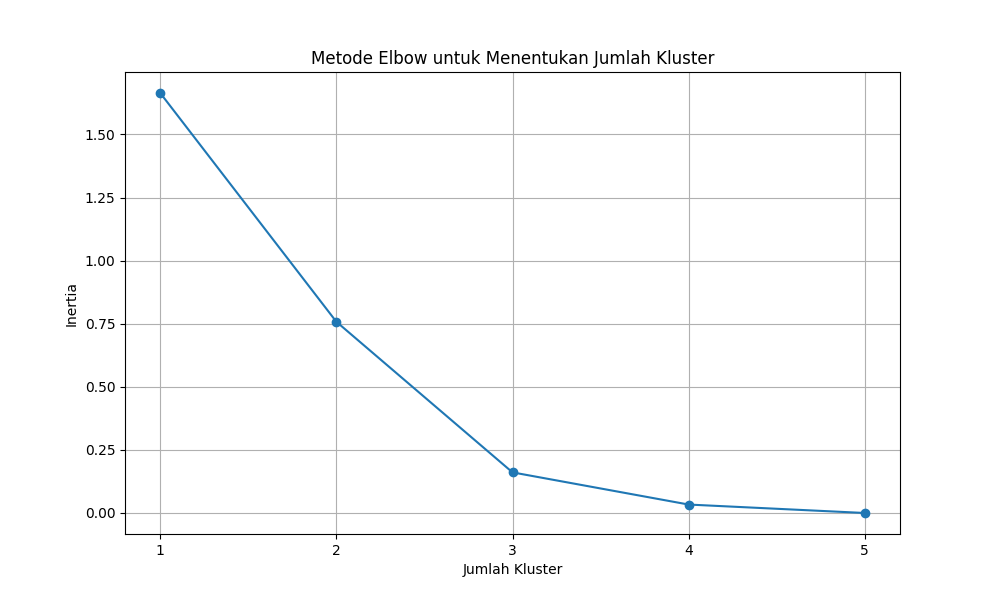
\includegraphics[width=0.7\linewidth]{images/elbow.png}
    \caption{Jumlah Kluster dengan metode Elbow}
    \label{fig:placeholder}
\end{figure}

Grafik Metode Elbow ini menunjukkan bahwa titik optimal untuk jumlah kluster dalam analisis K-means adalah 3. Pada titik ini, penurunan inertia mulai melambat, menunjukkan bahwa menambah kluster lebih dari 3 tidak memberikan pengurangan signifikansi dalam kesalahan kuadrat. Memilih 3 kluster memungkinkan pembagian data yang efisien tanpa overfitting, yang penting untuk analisis efektivitas program penyebaran bantuan sosial. Dengan kluster ini, Anda dapat mengidentifikasi kelompok masyarakat yang paling efektif mendapatkan manfaat dari bantuan, membantu dalam pengembangan strategi penanggulangan kemiskinan yang lebih tepat sasaran di Provinsi Bengkulu.

\begin{figure}[H]
    \centering
    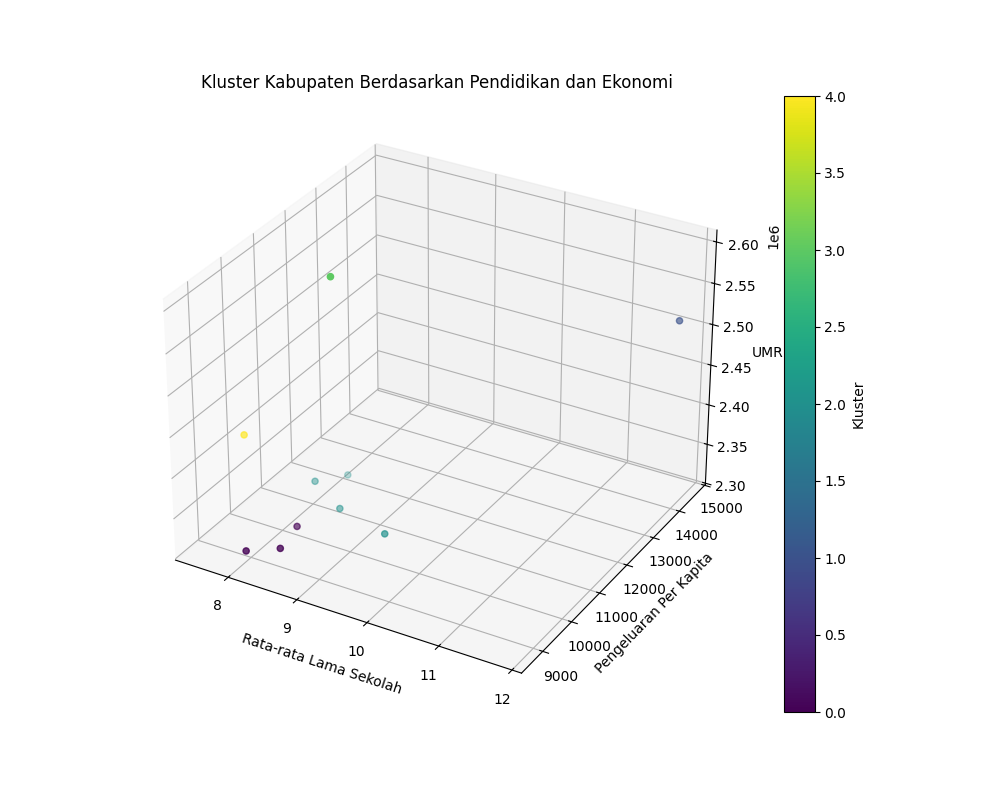
\includegraphics[width=0.7\linewidth]{images/hasil_kluster.png}
    \caption{Grafik Clustring }
    \label{fig:clustring}
\end{figure}

Berdasarkan Gambar \ref{fig:clustring} tersebut menunjukkan klasterisasi kabupaten berdasarkan variabel pendidikan dan ekonomi. Sumbu X menggambarkan rata-rata lama sekolah di setiap kabupaten, dengan rentang 8 hingga 12 tahun. Sumbu Y menunjukkan pengeluaran per kapita, dengan rentang antara 9000 hingga 15000. Sumbu Z menggambarkan Upah Minimum Regional (UMR), dengan nilai berkisar dari sekitar 2.30 hingga 2.60. Warna pada titik-titik menggambarkan kluster yang berbeda, yang mengelompokkan kabupaten berdasarkan kemiripan dalam tiga variabel tersebut. Warna yang berbeda menandakan kelompok yang berbeda. Dari analisis ini, terlihat bahwa kabupaten dengan rata-rata lama sekolah yang lebih tinggi cenderung memiliki pengeluaran per kapita yang lebih tinggi. Kenaikan UMR tampaknya tidak terlalu bervariasi di antara kluster, tetapi bisa memberikan sedikit perbedaan. Kluster yang lebih tinggi, ditunjukkan dengan warna lebih cerah, mungkin menunjukkan kabupaten dengan kondisi ekonomi dan pendidikan yang lebih baik. Penelitian lebih lanjut dapat dilakukan untuk memahami faktor-faktor penyebab perbedaan ini, dan bagaimana program bantuan sosial dapat dioptimalkan untuk kluster-kluster tertentu.

\begin{table}[h]
    \centering
    \begin{tabular}{ccccc}
        \hline
        \textbf{Kabupaten} & \textbf{Rata Rata Lama Sekolah} & \textbf{Pengeluaran Per Kapita} & \textbf{UMR} & \textbf{Kluster} \\
        \hline
        Bengkulu Selatan & 9.350 & 10,353.6 & 2,318,411.4 & 2 \\
        Rejang Lebong & 8.554 & 10,667.4 & 2,318,411.4 & 2 \\
        Bengkulu Utara & 8.098 & 10,870.0 & 2,334,301.4 & 2 \\
        Kaur & 8.404 & 9,069.4 & 2,318,411.4 & 0 \\
        Seluma & 8.070 & 8,711.2 & 2,318,411.4 & 0 \\
        Mukomuko & 8.406 & 10,831.6 & 2,594,047.4 & 3 \\
        Lebong & 8.216 & 11,691.8 & 2,318,411.4 & 2 \\
        Kepahiang & 8.312 & 9,804.4 & 2,318,411.4 & 0 \\
        Bengkulu Tengah & 7.532 & 9,869.2 & 2,410,581.4 & 4 \\
        Kota Bengkulu & 11.816 & 14,603.0 & 2,510,097.6 & 1 \\
        \hline
    \end{tabular}
    \caption{Data Kabupaten Bengkulu}
    \label{tab:data_hasil_cluster}
\end{table}

Berdasarkan Tabel \ref{tab:data_hasil_cluster} yang disajikan memberikan gambaran mengenai beberapa indikator sosial ekonomi dari berbagai kabupaten di Provinsi Bengkulu. Variabel yang dianalisis meliputi Rata-rata Lama Sekolah, Pengeluaran Per Kapita, Upah Minimum Regional (UMR), dan Kluster hasil analisis klustering. Rata-rata Lama Sekolah merupakan indikator penting yang mencerminkan tingkat pendidikan di setiap kabupaten. Pengeluaran Per Kapita memberikan wawasan tentang rata-rata pengeluaran individu per tahun, yang diukur dalam ribuan rupiah. UMR mencerminkan standar upah minimum yang berlaku di masing-masing kabupaten. Analisis klustering mengelompokkan kabupaten-kabupaten ini ke dalam beberapa kluster berdasarkan kesamaan karakteristik. Kluster 2, yang mencakup Bengkulu Selatan, Rejang Lebong, Bengkulu Utara, dan Lebong, menunjukkan pengeluaran per kapita yang relatif lebih tinggi. Sebaliknya, Kluster 0, terdiri dari Kaur, Seluma, dan Kepahiang, memiliki pengeluaran per kapita yang lebih rendah. Mukomuko, yang termasuk dalam Kluster 3, memiliki pengeluaran per kapita dan UMR yang tinggi, menempatkannya dalam kategori tersendiri. Bengkulu Tengah masuk ke Kluster 4 dengan pengeluaran per kapita menengah. Kota Bengkulu, yang berada di Kluster 1, menunjukkan rata-rata lama sekolah dan pengeluaran per kapita tertinggi di antara semua kabupaten. Dari analisis ini, dapat disimpulkan bahwa kabupaten dengan pengeluaran per kapita dan UMR lebih tinggi, seperti Kota Bengkulu, cenderung memiliki tingkat pendidikan yang lebih baik. Perbedaan antar kluster menunjukkan adanya variasi dalam kondisi sosial ekonomi, yang dapat menjadi dasar bagi penyesuaian kebijakan bantuan sosial untuk meningkatkan efektivitas dan efisiensi dalam penanggulangan kemiskinan di Provinsi Bengkulu.


\section{Kesimpulan dan Saran}

\subsection{Kesimpulan}

Kemiskinan di Provinsi Bengkulu merupakan permasalahan kompleks yang dipengaruhi oleh faktor pendidikan, ekonomi, dan kebijakan sosial. Indikator Rata-Rata Lama Sekolah (RLS), Pengeluaran Per Kapita, dan Upah Minimum Regional (UMR) menjadi tolok ukur penting dalam menilai efektivitas program bantuan sosial untuk mengurangi kemiskinan di daerah ini. 

Berdasarkan hasil analisis klasterisasi dengan metode K-Means, kabupaten-kabupaten di Bengkulu terbagi ke dalam beberapa kelompok berdasarkan karakteristik pendidikan dan ekonomi. Kabupaten dengan rata-rata lama sekolah dan pengeluaran per kapita yang lebih tinggi, seperti Kota Bengkulu, cenderung memiliki kondisi sosial ekonomi yang lebih baik dibandingkan kabupaten lainnya. 

Perbedaan kondisi sosial ekonomi antar kabupaten ini menunjukkan bahwa peningkatan kualitas pendidikan dan pendapatan memiliki peran signifikan dalam menekan tingkat kemiskinan. Variasi Upah Minimum Regional juga berpengaruh terhadap kesejahteraan masyarakat meskipun perbedaan UMR antar kabupaten tidak terlalu besar.

Hasil klasterisasi ini dapat menjadi dasar dalam penyusunan kebijakan bantuan sosial yang lebih tepat sasaran dan efektif, dengan menyesuaikan program sesuai karakteristik tiap kelompok kabupaten agar dampak penanggulangan kemiskinan menjadi maksimal.

\subsection{Saran}

\begin{enumerate}
    \item Pemerintah Provinsi Bengkulu disarankan untuk merancang program bantuan sosial yang lebih spesifik dan terfokus pada karakteristik masing-masing klaster kabupaten, agar alokasi sumber daya dapat lebih efektif.
    \item Peningkatan kualitas pendidikan melalui peningkatan akses dan mutu sekolah perlu diprioritaskan sebagai strategi utama dalam menekan angka kemiskinan jangka panjang.
    \item Perlu adanya upaya untuk meningkatkan pengeluaran per kapita masyarakat, misalnya melalui pelatihan keterampilan dan peningkatan kesempatan kerja.
    \item Pemerintah juga sebaiknya mengkaji kebijakan Upah Minimum Regional agar lebih responsif terhadap kebutuhan ekonomi masyarakat, khususnya di kabupaten dengan UMR yang lebih rendah.
    \item Penelitian lanjutan disarankan untuk menggali faktor-faktor lain yang mempengaruhi kemiskinan di Bengkulu agar penanggulangan dapat dilakukan secara lebih komprehensif.
\end{enumerate}



\clearpage
\renewcommand{\refname}{Daftar Pustaka}
\bibliographystyle{johd}
\bibliography{bib}


\end{document}